\documentclass[twocolumn]{article}
\usepackage{amsmath}
\usepackage{xcolor}
\usepackage{graphicx}
\usepackage{caption}
\usepackage{fancyhdr}
\usepackage{geometry}
\usepackage{enumitem}
\usepackage{array}
\usepackage{hyperref}
\geometry{margin=0.7in}
\pagestyle{empty}

\begin{document}

\begin{figure}[t]
    
\includegraphics[width=\linewidth]{img3.png} % Use uploaded image
                \textbf{Name: K.Saisusmitha} \\
    \textbf{Batch: 2} \\
    \textbf{ID: cometfwc018} \\
    \textbf{Date: 9th July 2025}
\end{figure}

\begin{center}
    {\LARGE \textbf{\textcolor{blue}{GATE Question Paper 2010, IN Question Number 42}}}
\end{center}

\vspace{1em}
\begin{figure}[h]
    \centering
    \includegraphics[width=0.8\linewidth]{in2010 42.png}
    \caption*{\textbf{Figure: Logic Gate Circuit}}
\end{figure}

\section*{\textcolor{blue}{Question Analysis}}
\textbf{Given:} A combinational logic gate circuit using NOT, AND, and OR gates with inputs $X$ and $Y$.  
\textbf{Task:} Identify the overall logic function $Z$.

\section*{Solution:}

\begin{enumerate}[label=\textbf{Step \arabic*:}]
    \item \textbf{Label Gate Outputs for Clarity:}
    \begin{itemize}
        \item Let $A = \overline{X}$ and $B = \overline{Y}$
        \item $C = X \cdot B = X \cdot \overline{Y}$
        \item $D = A \cdot Y = \overline{X} \cdot Y$
        \item $Z = C + D$
    \end{itemize}

    \item \textbf{Combine Logic:}
    \[
    Z = (X \cdot \overline{Y}) + (\overline{X} \cdot Y)
    \]

    \item \textbf{Recognize Logic Pattern:}
    \[
    Z = X \oplus Y
    \]
    This is the standard definition of the XOR operation.
\end{enumerate}

\section*{\textcolor{blue}{Correct Option: (A) XOR}}

\section*{\textcolor{blue}{Truth Table}}
\begin{table}[h]
\centering
\renewcommand{\arraystretch}{1.3}
\begin{tabular}{|c|c|c|c|c|}
\hline
X & Y & $\overline{X}$ & $\overline{Y}$ & Z = $X \oplus Y$ \\
\hline
0 & 0 & 1 & 1 & 0 \\
0 & 1 & 1 & 0 & 1 \\
1 & 0 & 0 & 1 & 1 \\
1 & 1 & 0 & 0 & 0 \\
\hline
\end{tabular}
\caption*{\textbf{Table: Truth Table for the Logic Circuit}}
\end{table}

\section*{\textcolor{blue}{Hardware Implementation}}

\textbf{Logic Expression:} $Z = X \oplus Y$

\textbf{Inputs:} $X$, $Y$ – Push buttons  
\textbf{Output:} $Z$ – LED indicates result

\subsection*{\textcolor{blue}{Hardware Requirements}}

\begin{table}[h]
\centering
\renewcommand{\arraystretch}{1.3}
\begin{tabular}{|c|l|}
\hline
\textbf{S.No} & \textbf{Component} \\ \hline
1 & Pico2W or Arduino Uno \\
2 & Breadboard \\
3 & Push Buttons (2x) for X and Y \\
4 & LED for Output Z \\
5 & Resistors (220$\Omega$ for LED, 10k$\Omega$ for pull-downs) \\
6 & Jumper Wires \\
7 & USB Cable \\
\hline
\end{tabular}
\caption*{\textbf{Required Components for XOR Circuit}}
\end{table}

\subsection*{\textcolor{blue}{GPIO Pin Mapping (Pico2W)}}

\begin{table}[h]
\centering
\renewcommand{\arraystretch}{1.3}
\begin{tabular}{|c|c|c|}
\hline
\textbf{Component} & \textbf{Pico2W Pin} & \textbf{Description} \\
\hline
Button X & GP14 & Input X \\
Button Y & GP15 & Input Y \\
LED (Output Z) & GP13 & Output XOR \\
GND & GND & Common Ground \\
3.3V & 3.3V & Pull-up Voltage \\
\hline
\end{tabular}
\end{table}

\subsection*{\textcolor{blue}{Arduino Uno GPIO Mapping}}

\begin{table}[h]
\centering
\renewcommand{\arraystretch}{1.3}
\begin{tabular}{|c|c|c|}
\hline
\textbf{Component} & \textbf{Arduino Pin} & \textbf{Description} \\
\hline
Button X & D2 & Input X \\
Button Y & D3 & Input Y \\
LED Z & D6 & Output (XOR) \\
GND & GND & Ground \\
VCC & 5V & Power \\
\hline
\end{tabular}
\end{table}

\subsection*{\textcolor{blue}{Testing Procedure}}
\begin{enumerate}
    \item Power up board and connect circuit.
    \item Press combinations of $X$ and $Y$:
    \begin{itemize}
        \item 00 → Z = 0
        \item 01 → Z = 1
        \item 10 → Z = 1
        \item 11 → Z = 0
    \end{itemize}
    \item Verify LED glows only for XOR condition.
\end{enumerate}

\section*{\textcolor{blue}{Conclusion}}
\begin{figure}[h]
    \centering
    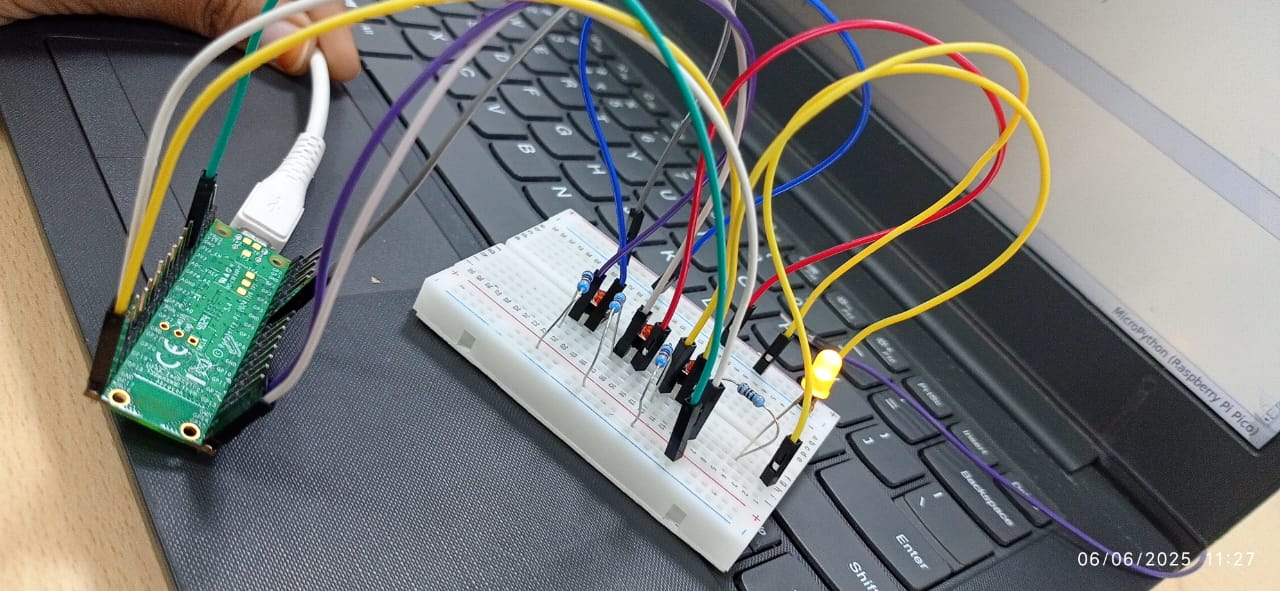
\includegraphics[width=0.9\linewidth]{Assembly.jpg}
        \caption*{\textbf{Figure: XOR Implementation Setup (Representative)}}
\end{figure}

The given logic gate network implements the function:
\[
Z = X \cdot \overline{Y} + \overline{X} \cdot Y = X \oplus Y
\]
Hence, the correct answer is:
\[
\boxed{\text{(A) XOR}}
\]

\section*{\textcolor{blue}{Source Code Link}}
The complete hardware simulation and code implementation for this experiment is available at the following GitHub repository:

\textbf{GitHub Repo:} \href{https://github.com/aisusmitha/FWC.git}{github.com/aisusmitha/FWC.git}

\end{document}
